
\documentclass{beamer}

\usetheme{Copenhagen}

\title{Matrix Project}
\subtitle{EE1390- Intro to AI and ML}
\usepackage{graphicx}
\graphicspath{{./images/}}

\author{
Md.Sadiq -  \
\texttt{EE18BTECH11051}
\and \\
S.Abdur Rahman Nawaz -  \
\texttt{EE18BTECH11052}
}
\institute{IIT HYDERABAD}
\date{February 15, 2019}

\subject{JEE questions solving using python}

\AtBeginSubsection[]
{
  \begin{frame}<beamer>{Outline}
    \tableofcontents[currentsection,currentsubsection]
  \end{frame}
}

\begin{document}

\begin{frame}
  \titlepage
\end{frame}

\begin{frame}{Outline}
  \tableofcontents
\end{frame}

\section{Problem Statement}

\begin{frame}{IIT JEE 2005 Question}
 
 
   Q.Tangent to the curve $y = x^2 + 6$ at a point (1,7) touches the circle $x^2 + y^2 + 16x + 12y + k = 0$. Then the Coordinates of Q are \\
  (a) (-6, -11)\\
  (b) (-9, -13)\\
  (c) (10, -15)\\
  (d) (-6, -7)\\
\end{frame}

\section{Solution}

\begin{frame}{Solution}

\begin{center}
    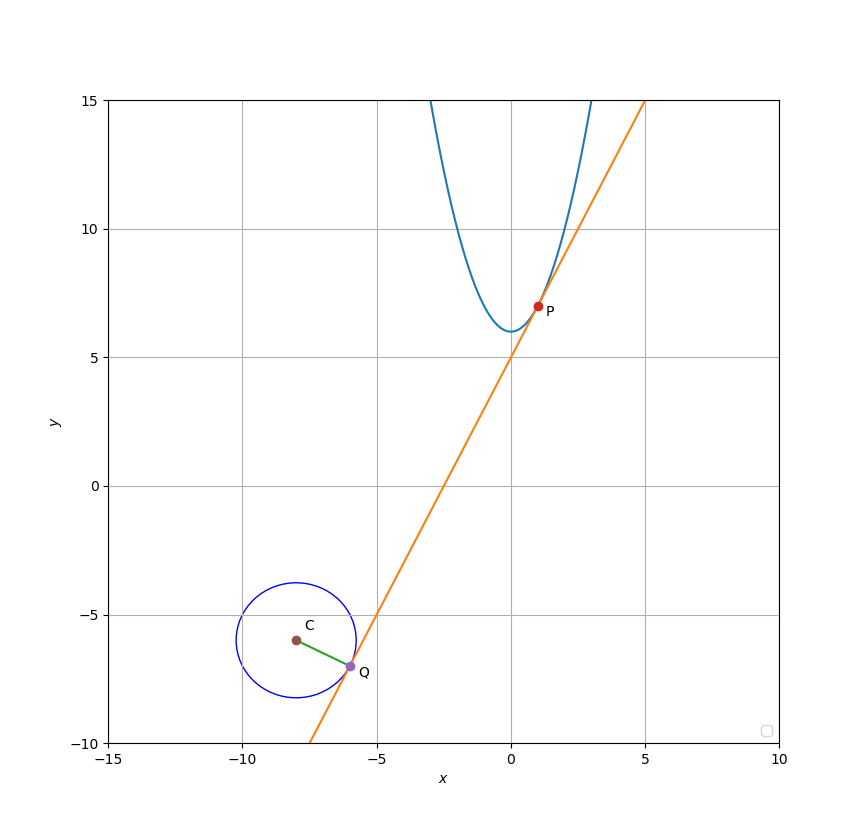
\includegraphics[scale =0.35]{Fig1.png}
\end{center}



\end{frame}

\begin{frame}{Solution}
The given parabola equation is \\
\begin{equation}
y = x^2 + 6 => x^2 - y + 6 = 0  
\end{equation}
writing it in matrix form
\begin{equation}
 \mathbf{x}^\intercal\begin{pmatrix} 1 \ 0 \\ 0 \ 0 \end{pmatrix}\mathbf{x} + \begin{pmatrix} 0 \\ -1 \end{pmatrix}\mathbf{x} + 6 = 0
\end{equation}
Equation of a standard second order conic is
\begin{equation}
    \mathbf{x}^\intercal\mathbf{V}\mathbf{x} + 2\mathbf{U}^\intercal\mathbf{x} + F = 0
\end{equation}
On comparing
\begin{equation}
 V = \begin{pmatrix} 1 \ 0 \\ 0 \ 0 \end{pmatrix} \  U = \begin{pmatrix} 0 \ -1/2 \end{pmatrix}  and\ F = 6  
\end{equation}

\end{frame}

\begin{frame}{Solution}
And for a standard second order conic the equation of tangent at P is 
\begin{equation}
    (\mathbf{P}^\intercal\mathbf{V} + \mathbf{U}^\intercal)\mathbf{x} + \mathbf{P}^\intercal\mathbf{U} + F = 0
\end{equation}
And now substituting all the values the equation of tangent is 
\begin{equation}
    \begin{pmatrix} -2 \ 1 \end{pmatrix}\mathbf{x} = 5
\end{equation}
Any equation of a circle is given as
\begin{equation}
    ||x-c||^{2} = r^2
\end{equation}
\begin{equation}
    (\mathbf{x-c})^\intercal(\mathbf{x-c}) = r^2
\end{equation}
\begin{equation}
    \mathbf{x}^\intercal\mathbf{x} - 2\mathbf{c}\mathbf{x} = r^2 - \mathbf{c}^\intercal\mathbf{c}
\end{equation}
\end{frame}

\begin{frame}{Solution}
On comparing it with the given equation
\begin{equation}
  x^2 + y^2 + 16x + 12y + k = 0  
\end{equation}
Centre of the circle c is
\begin{equation}
    c = \begin{pmatrix} -8 \\ -6 \end{pmatrix}
\end{equation}
\begin{center}
      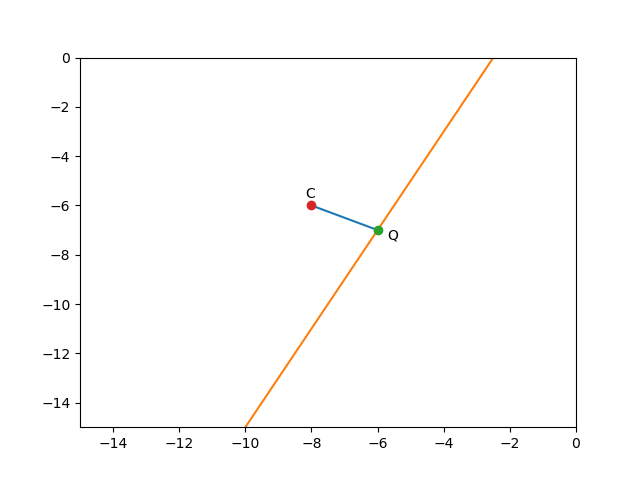
\includegraphics[scale =0.35]{Fig2.png}
\end{center}

\end{frame}

\begin{frame}{Solution}
Equation of tangent $\mathbf{n_{1}}\mathbf{x} = p_{1}$\\
Equation of a line perpendicular to tangent and passing through c is,
\begin{equation}
    \mathbf{n_{2}}(\mathbf{x} - \mathbf{c}) = 0
\end{equation}
Where $\mathbf{n_{2}}$ can be easily calculated using $\mathbf{n_{1}}$ and orthogonal matrix\\

Which can be written as 
\begin{equation}
\mathbf{n_{2}}\mathbf{x} = p_{2} \ where\ p_{2} = \mathbf{n_{2}}\mathbf{c} 
\end{equation}
 
And then the point Q is the intersection of both the lines i.e the Tangent and the Normal
Which gives  $ Q = (-6, -7) $ 
    
\end{frame}

\section{Graphical representation}

\begin{frame}{Graphical representation}
\begin{center}
   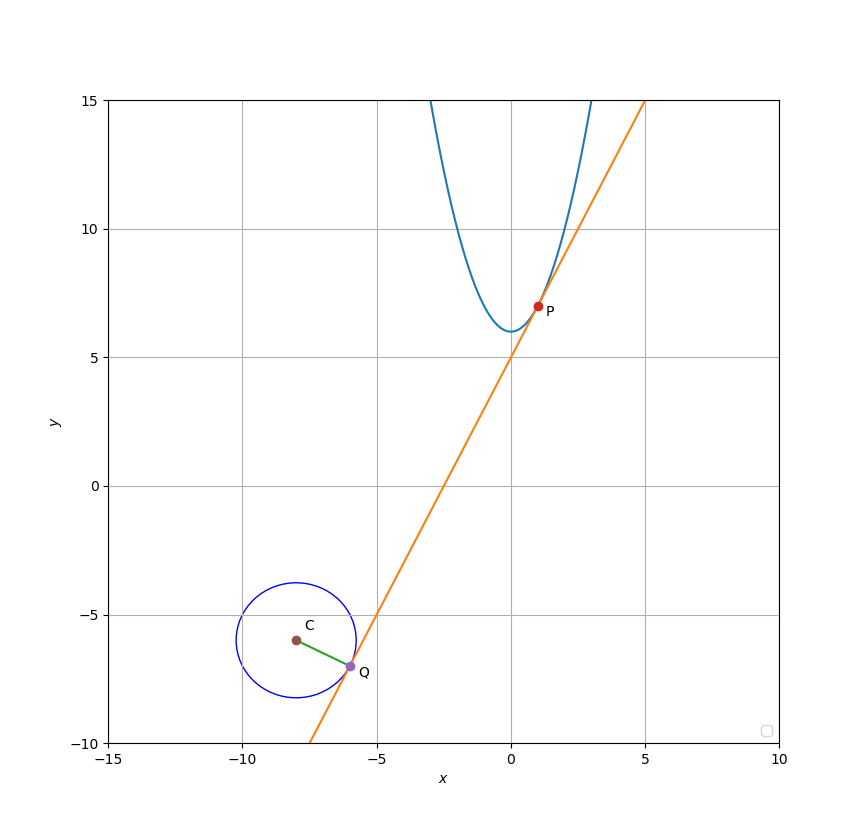
\includegraphics[scale =0.35]{Fig1.png} 
\end{center}

 
\end{frame}

\begin{frame}{Final Slide}
\begin{center}
    THANK YOU
\end{center}
    
\end{frame}
    

\end{document}


